%% LyX 2.4.4 created this file.  For more info, see https://www.lyx.org/.
%% Do not edit unless you really know what you are doing.
\documentclass[english]{article}
\usepackage[T1]{fontenc}
\usepackage[latin9]{inputenc}
\usepackage{float}
\usepackage{enumitem}
\usepackage{amsmath}
\usepackage{amsthm}
\usepackage{cancel}
\usepackage{geometry}
\geometry{verbose,tmargin=1in,bmargin=1in,lmargin=1in,rmargin=1in}

\makeatletter

%%%%%%%%%%%%%%%%%%%%%%%%%%%%%% LyX specific LaTeX commands.
%% Because html converters don't know tabularnewline
\providecommand{\tabularnewline}{\\}

%%%%%%%%%%%%%%%%%%%%%%%%%%%%%% Textclass specific LaTeX commands.
\numberwithin{equation}{section}
\numberwithin{figure}{section}
\newlength{\lyxlabelwidth}      % auxiliary length 

%%%%%%%%%%%%%%%%%%%%%%%%%%%%%% User specified LaTeX commands.
\usepackage{hyperref}
\usepackage[usenames,dvipsnames,table]{xcolor} %adds additional color options
\hypersetup{colorlinks=true, urlcolor=black,linkcolor=black}

\usepackage{fancyhdr}
\usepackage{lastpage}
\pagestyle{fancy}
\usepackage{enumitem}
\usepackage{ifthen}
%sets math fonts to be more readable
%\everymath=\expandafter{\the\everymath\displaystyle}
%\DeclareMathSizes{10}{10}{10}{10}
\usepackage{multicol}

\usepackage{tikz}
\usetikzlibrary{plotmarks}
\usepackage{pgfplots}
\pgfplotsset{compat=newest}

\usepackage{calc}
\usepackage[nomessages]{fp}

\usepackage{advdate}    % Advancing/saving dates
\usepackage{datetime}   % Dates formatting
\usepackage{datenumber} % Counters for dates

\usepackage{fancybox} %%ovalbox and fancy box settings

\usepackage[super]{nth} %easy 1st, 2nd, etc

\usepackage{forest} %%for tree diagram

%%data for histogram%%
\begin{filecontents}{hist1_data.csv} 
dist 
3
1
0
4
1
3
2
2
0
2
0
2
2
1
4
3
1
1
3
4
2
1
3
0
1
0
2
5
1
2
3
0
0
1
2
3
1
2
0
2
\end{filecontents}

%%data for histogra: cal per cereal%%
\begin{filecontents}{hist_data_cereal.csv} 
dist 
3.7
3.6
3.6
4.0
4.0
3.6
3.8
3.7
4.1
3.9
3.9
3.3
3.5
3.6
3.9
4.0
\end{filecontents}
% Added by lyx2lyx
\setlength{\parskip}{\smallskipamount}
\setlength{\parindent}{0pt}

\makeatother

\usepackage{babel}
\begin{document}
\renewcommand{\author}{Dr.\,James Ashe}

\newcommand{\classNum}{107}

\newcommand{\classSec}{7 and 10}

\newcommand{\nameType}{Solutions}

\newcommand{\examType}{Exam 4}

\renewcommand{\date}{ \formatdate{21}{11}{2014}}

%%First page's header%%%%%%%%%%%%%%%%%%%%%%
\fancypagestyle{firststyle} %%header settings for first pagr
{
	\fancyhead[L]{MTH \classNum{}(\classSec{}) \author{}\\
	\textbf{\examType{}} \date{}}
	\fancyhead[C]{\textbf{\nameType}}
	\setlength{\headsep}{14pt}
}
%%%%%%%%%%%%%%%%%%%%%%%%%%%%%%%%%%%%%%%%%%

%%Next page's header%%%%%%%%%%%%%%%%%%%%%%%
%\setlist{nolistsep}
\lhead{MTH \classNum{}(\classSec{})} 
\chead{\textbf{\nameType}} 
\cfoot{\thepage{}~of~\pageref{LastPage}} 
\setlength{\headsep}{5pt} 
%%%%%%%%%%%%%%%%%%%%%%%%%%%%%%%%%%%%%%%%%%%

%%Various settings; see the preamble for other settings%%%%%
%%\setenumerate[0]{leftmargin=12pt,itemindent=0pt,labelwidth=0pt}
%\setlist[2]{noitemsep}
%\setlist{nosep}
\setlist{itemsep=-3pt,topsep=-2pt}
\renewcommand{\labelenumi}{\textbf{\arabic{enumi}.}}
\renewcommand{\labelenumii}{\textbf{\alph{enumii}.}}
\thispagestyle{firststyle}
%%%%%%%%%%%%%%%%%%%%%%%%%%%%%%%%%%%%%%%%%%
\newcommand{\xmax}{10}
\newcommand{\xmin}{-10}
\newcommand{\xstep}{0} %must be xmin+n
\newcommand{\ymax}{10}
\newcommand{\ymin}{-10}
\newcommand{\ystep}{0} %must be ymin+n

\newcommand{\xspace}{\hspace*{40pt}}
\newcommand{\yspace}{\vspace*{1.4cm}}
\newcommand{\rowColor}{gray!35}
\large

\newcommand{\gauss}[2]{1/(#2*sqrt(2*pi))*exp(-((x-#1)^2)/(2*#2^2))}

\newcommand{\normalcdf}[4]{ %mean,std,z-left,z-right
\begin{tikzpicture}[scale=1.25]

\pgfmathsetmacro{\mn}{#1}
\pgfmathsetmacro{\sd}{#2}
\pgfmathsetmacro{\za}{#1+#2*1}
\pgfmathsetmacro{\zb}{#1+#2*2}
\pgfmathsetmacro{\zc}{#1+#2*3}

\pgfmathsetmacro{\zna}{#1-#2*1}
\pgfmathsetmacro{\znb}{#1-#2*2}
\pgfmathsetmacro{\znc}{#1-#2*3}

\pgfmathsetmacro{\zleft}{#3}
\pgfmathsetmacro{\zright}{#4}
\pgfmathsetmacro{\zsL}{(#3-#1)/#2} %z-score
\pgfmathsetmacro{\zsR}{(#4-#1)/#2} %z-score
\pgfmathsetmacro{\xCenter}{\zsL/2.5+\zsR/2.5} %center using z-score
\pgfmathsetmacro{\yCenter}{((1/(1*sqrt(2*pi))*exp(-((\xCenter-0)^2)/(2*1^2)))/2}
\pgfkeys{/pgf/fpu} %for large numbers
\pgfmathparse{100*(1/(1 + exp(-0.07056*((\zsR-0)/1)^3 - 1.5976*(\zsR-0)/1))-1/(1 + exp(-0.07056*((\zsL-0)/1)^3 - 1.5976*(\zsL-0)/1)))} %area from z-left to z-right
\edef\area{\pgfmathresult} 
\pgfkeys{/pgf/fpu=false}

\scriptsize
\begin{axis}[ 
	no markers, 
	domain=0:10, 
	%samples=100, 
	axis lines*=left, 
	%xlabel=Standard deviations, 
	%ylabel=Frequency, 
	height=2.5cm, %change/remove this scaling to get 1:1 pic
	width=5.5cm, 
	hide y axis,
	%ticks=none,
	xtick={-3,-2,-1,0,1,2,3},
	xticklabels={\pgfmathprintnumber[precision=0]{\znc},\pgfmathprintnumber[precision=2]{\znb},\pgfmathprintnumber[precision=2]{\zna},#1,\pgfmathprintnumber[precision=0]{\za},\pgfmathprintnumber[precision=2]{\zb},\pgfmathprintnumber[precision=2]{\zc}},
	%xticklabels={-25, -15, -5, 5, 15, 25, 35},
	%ytick=empty, 
	enlargelimits=false, 
	clip=false, 
	axis on top, 
	%grid = major
	]

	\addplot [fill=blue!35, draw=red,  domain=\zsL:\zsR] {\gauss{0}{1}} \closedcycle;
		\node (arrowEnd) at (axis cs: \xCenter, \yCenter) {};
	\addplot [draw, thick, smooth, domain=-3:3] {\gauss{0}{1}} \closedcycle;
		\node[anchor=south east] (arrowStart) at (current bounding box.east) {\pgfmathprintnumber[fixed,precision=1]{\area}\%};
	\draw[->,thick,black] (arrowStart) to (arrowEnd);
	
	%\addplot [fill=orange!20, draw=none, domain=2:3] {\gauss{0}{1}} \closedcycle; 
	%\addplot [fill=blue!20, draw=none, domain=-2:-1] {\gauss{0}{1}} \closedcycle; 
	%\addplot [fill=blue!20, draw=none, domain=1:2] {\gauss{0}{1}} \closedcycle; 
	%\only<1->{\node[above] at (axis cs: -0.5, 0.025) {$34.1\%$};} 
	%\only<1->{\node[above] at (axis cs: 0.5, 0.025) {$34.1\%$};} 
	%\only<1->{\node[above] at (axis cs: -1.5, 0.025) {$13.6\%$};}
	%\only<1->{\node[above] at (axis cs: 1.5, 0.025) {$13.6\%$};}
	%\only<1->{\node[above] at (axis cs: 2.5, 0.05) {$2.1\%$};}
	%\only<1->{\node[above] at (axis cs: -2.5, 0.05) {$2.1\%$};}
	%\only<1->{ \addplot[<->,black,very thick] coordinates {(-1,0.4) (1,0.4)};} 
	%\only<1->{\node[above] at (axis cs: 0, 0.4) {$68.2\%$};} 
	%\only<1->{\addplot[<->,black,very thick] coordinates {(-2,0.3) (2,0.3)};}
	%\only<1->{\node[above] at (axis cs: 0, 0.3) {$95.4\%$};}
	%\only<1->{\addplot[<->,black, very thick] coordinates {(-3,0.2) (3,0.2)};} 
	%\only<1->{\node[above] at (axis cs: 0, 0.2) {$99.7\%$};}
	\end{axis} 
\end{tikzpicture}
}

\newcommand{\normalpdf}[5]{ %mean,std,z-left,z-right
\begin{tikzpicture}[scale=1.25]

\pgfmathsetmacro{\mn}{#1}
\pgfmathsetmacro{\sd}{#2}
\pgfmathsetmacro{\za}{#1+#2*1}
\pgfmathsetmacro{\zb}{#1+#2*2}
\pgfmathsetmacro{\zc}{#1+#2*3}

\pgfmathsetmacro{\zna}{#1-#2*1}
\pgfmathsetmacro{\znb}{#1-#2*2}
\pgfmathsetmacro{\znc}{#1-#2*3}

\pgfmathsetmacro{\zleft}{#3}
\pgfmathsetmacro{\zright}{#4}
\pgfmathsetmacro{\zsL}{(#3-#1)/#2} %z-score
\pgfmathsetmacro{\zsR}{(#4-#1)/#2} %z-score
\pgfmathsetmacro{\zsV}{(#5-#1)/#2} %z-score
\pgfmathsetmacro{\xCenter}{\zsL/2.5+\zsR/2.5} %center using z-score
\pgfmathsetmacro{\yCenter}{((1/(1*sqrt(2*pi))*exp(-((\xCenter-0)^2)/(2*1^2)))/2}
\pgfkeys{/pgf/fpu} %for large numbers
\pgfmathparse{100*(1/(1 + exp(-0.07056*((\zsR-0)/1)^3 - 1.5976*(\zsR-0)/1))-1/(1 + exp(-0.07056*((\zsL-0)/1)^3 - 1.5976*(\zsL-0)/1)))} %area from z-left to z-right
\edef\area{\pgfmathresult} 
\pgfkeys{/pgf/fpu=false}

\scriptsize
\begin{axis}[ 
	no markers, 
	domain=0:10, 
	%samples=100, 
	axis lines*=left, 
	%xlabel=Standard deviations, 
	%ylabel=Frequency, 
	height=2.5cm, %change/remove this scaling to get 1:1 pic
	width=5.5cm, 
	hide y axis,
	%ticks=none,
	xtick={\zsV},
	xticklabels={\pgfmathprintnumber[precision=2]{#5}},
	%xticklabels={-25, -15, -5, 5, 15, 25, 35},
	%ytick=empty, 
	enlargelimits=false, 
	clip=false, 
	axis on top, 
	%grid = major
	]

	\addplot [fill=blue!35, draw=red,  domain=\zsL:\zsR] {\gauss{0}{1}} \closedcycle;
		\node (arrowEnd) at (axis cs: \xCenter, \yCenter) {};
	\addplot [draw, thick, smooth, domain=-3:3] {\gauss{0}{1}} \closedcycle;
		\node[anchor=south east] (arrowStart) at (current bounding box.east) {\pgfmathprintnumber[fixed,precision=1]{\area}\%};
	\draw[->,thick,black] (arrowStart) to (arrowEnd);
	
	%\addplot [fill=orange!20, draw=none, domain=2:3] {\gauss{0}{1}} \closedcycle; 
	%\addplot [fill=blue!20, draw=none, domain=-2:-1] {\gauss{0}{1}} \closedcycle; 
	%\addplot [fill=blue!20, draw=none, domain=1:2] {\gauss{0}{1}} \closedcycle; 
	%\only<1->{\node[above] at (axis cs: -0.5, 0.025) {$34.1\%$};} 
	%\only<1->{\node[above] at (axis cs: 0.5, 0.025) {$34.1\%$};} 
	%\only<1->{\node[above] at (axis cs: -1.5, 0.025) {$13.6\%$};}
	%\only<1->{\node[above] at (axis cs: 1.5, 0.025) {$13.6\%$};}
	%\only<1->{\node[above] at (axis cs: 2.5, 0.05) {$2.1\%$};}
	%\only<1->{\node[above] at (axis cs: -2.5, 0.05) {$2.1\%$};}
	%\only<1->{ \addplot[<->,black,very thick] coordinates {(-1,0.4) (1,0.4)};} 
	%\only<1->{\node[above] at (axis cs: 0, 0.4) {$68.2\%$};} 
	%\only<1->{\addplot[<->,black,very thick] coordinates {(-2,0.3) (2,0.3)};}
	%\only<1->{\node[above] at (axis cs: 0, 0.3) {$95.4\%$};}
	%\only<1->{\addplot[<->,black, very thick] coordinates {(-3,0.2) (3,0.2)};} 
	%\only<1->{\node[above] at (axis cs: 0, 0.2) {$99.7\%$};}
	\end{axis} 
\end{tikzpicture}
}\newcommand{\normalpdfB}[4]{ %mean,std,z-left,z-right
\begin{tikzpicture}[scale=1.25]

\pgfmathsetmacro{\mn}{#1}
\pgfmathsetmacro{\sd}{#2}
\pgfmathsetmacro{\za}{#1+#2*1}
\pgfmathsetmacro{\zb}{#1+#2*2}
\pgfmathsetmacro{\zc}{#1+#2*3}

\pgfmathsetmacro{\zna}{#1-#2*1}
\pgfmathsetmacro{\znb}{#1-#2*2}
\pgfmathsetmacro{\znc}{#1-#2*3}

\pgfmathsetmacro{\zleft}{#3}
\pgfmathsetmacro{\zright}{#4}
\pgfmathsetmacro{\zsL}{(#3-#1)/#2} %z-score
\pgfmathsetmacro{\zsR}{(#4-#1)/#2} %z-score
\pgfmathsetmacro{\xCenter}{\zsL/2.5+\zsR/2.5} %center using z-score
\pgfmathsetmacro{\yCenter}{((1/(1*sqrt(2*pi))*exp(-((\xCenter-0)^2)/(2*1^2)))/2}
\pgfkeys{/pgf/fpu} %for large numbers
\pgfmathparse{100*(1/(1 + exp(-0.07056*((\zsR-0)/1)^3 - 1.5976*(\zsR-0)/1))-1/(1 + exp(-0.07056*((\zsL-0)/1)^3 - 1.5976*(\zsL-0)/1)))} %area from z-left to z-right
\edef\area{\pgfmathresult} 
\pgfkeys{/pgf/fpu=false}

\scriptsize
\begin{axis}[ 
	no markers, 
	domain=0:10, 
	%samples=100, 
	axis lines*=left, 
	%xlabel=Standard deviations, 
	%ylabel=Frequency, 
	height=2.5cm, %change/remove this scaling to get 1:1 pic
	width=5.5cm, 
	hide y axis,
	%ticks=none,
	xtick={\zsL,\zsR},
	xticklabels={\pgfmathprintnumber[precision=2]{\zsL},\pgfmathprintnumber[precision=2]{\zsR}},
	%xticklabels={-25, -15, -5, 5, 15, 25, 35},
	%ytick=empty, 
	enlargelimits=false, 
	clip=false, 
	axis on top, 
	%grid = major
	]

	\addplot [fill=blue!35, draw=red,  domain=\zsL:\zsR] {\gauss{0}{1}} \closedcycle;
		\node (arrowEnd) at (axis cs: \xCenter, \yCenter) {};
	\addplot [draw, thick, smooth, domain=-3:3] {\gauss{0}{1}} \closedcycle;
		\node[anchor=south east] (arrowStart) at (current bounding box.east) {\pgfmathprintnumber[fixed,precision=1]{\area}\%};
	\draw[->,thick,black] (arrowStart) to (arrowEnd);
	
	%\addplot [fill=orange!20, draw=none, domain=2:3] {\gauss{0}{1}} \closedcycle; 
	%\addplot [fill=blue!20, draw=none, domain=-2:-1] {\gauss{0}{1}} \closedcycle; 
	%\addplot [fill=blue!20, draw=none, domain=1:2] {\gauss{0}{1}} \closedcycle; 
	%\only<1->{\node[above] at (axis cs: -0.5, 0.025) {$34.1\%$};} 
	%\only<1->{\node[above] at (axis cs: 0.5, 0.025) {$34.1\%$};} 
	%\only<1->{\node[above] at (axis cs: -1.5, 0.025) {$13.6\%$};}
	%\only<1->{\node[above] at (axis cs: 1.5, 0.025) {$13.6\%$};}
	%\only<1->{\node[above] at (axis cs: 2.5, 0.05) {$2.1\%$};}
	%\only<1->{\node[above] at (axis cs: -2.5, 0.05) {$2.1\%$};}
	%\only<1->{ \addplot[<->,black,very thick] coordinates {(-1,0.4) (1,0.4)};} 
	%\only<1->{\node[above] at (axis cs: 0, 0.4) {$68.2\%$};} 
	%\only<1->{\addplot[<->,black,very thick] coordinates {(-2,0.3) (2,0.3)};}
	%\only<1->{\node[above] at (axis cs: 0, 0.3) {$95.4\%$};}
	%\only<1->{\addplot[<->,black, very thick] coordinates {(-3,0.2) (3,0.2)};} 
	%\only<1->{\node[above] at (axis cs: 0, 0.2) {$99.7\%$};}
	\end{axis} 
\end{tikzpicture}
}

\emph{Unless stated otherwise, all problems are worth equal value
and answers should be stated as decimals rounded to three decimal
places. You must show your work to receive credit. }
\begin{enumerate}[resume]
\item Use figure \ref{fig:Number-of-children} to complete the following.\begin{multicols}{2}

\begin{enumerate}
\item Create a frequency distribution table from figure \ref{fig:Number-of-children}
(approximate).

\begin{enumerate}
\item []\Large%
\begin{tabular}{c|c|c|}
\cline{2-3}
mid & \textbf{hours} & \textbf{freq.}\tabularnewline
\cline{2-3}
13 & $12\leq x<14$ & 12\tabularnewline
\cline{2-3}
15 & $14\leq x<16$ & 17\tabularnewline
\cline{2-3}
17 & $16\leq x<18$ & 13\tabularnewline
\cline{2-3}
19 & $18\leq x<20$ & 5\tabularnewline
\cline{2-3}
21 & $20\leq x<22$ & 3\tabularnewline
\cline{2-3}
\multicolumn{1}{c}{} & \multicolumn{1}{c}{total} & \multicolumn{1}{c}{50}\tabularnewline
\end{tabular}\normalsize\vspace{10pt}
\end{enumerate}
\item Using your frequency table, find the mean.

\begin{enumerate}
\item []$\bar{x}=\frac{13\cdot12+15\cdot17+17\cdot13+19\cdot5+21\cdot3}{50}$\\
\hspace{0cm}\hphantom{$\bar{x}$ }$=\frac{790}{50}=15.8$\vfill
\end{enumerate}
\item What percentage of students are taking less than 14 hours?

\begin{enumerate}
\item []$\frac{12}{50}=24\%$\vfill\columnbreak
\end{enumerate}
\item []
\begin{figure}[H]
\begin{centering}
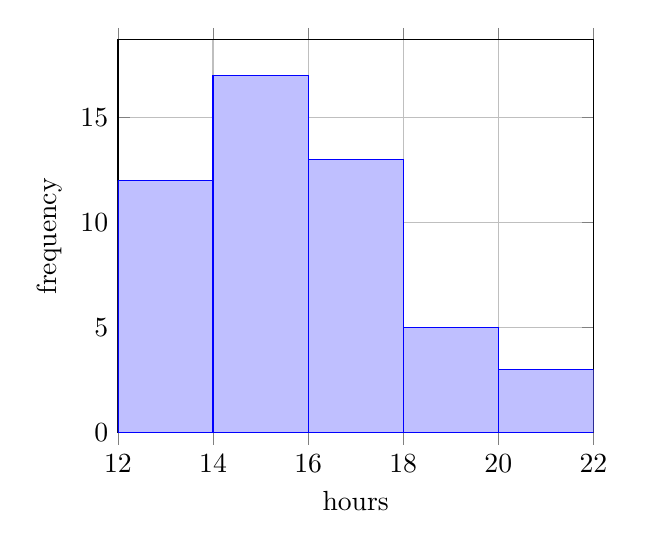
\begin{tikzpicture}[scale=1]
\begin{axis}[     
	ybar interval,
	x tick label as interval=false,    
	ymin=0,
	xmin=12,
	xmax=22,
	width=3in,
	%height=3in,
	grid=major,
	ylabel=frequency,
	xlabel=hours
	] 
	\addplot [fill=blue!25,draw=blue] table [x=Lower, y=Count] { 
		Lower Upper Count 
		12	14	12
		14	16	17
		16	18	13
		18	20	5
		20	22	3
		22	24	0
	};
\end{axis}
\end{tikzpicture}
\par\end{centering}
\caption{\label{fig:Number-of-children}Credit hours of 50 students.}
\end{figure}
\yspace\yspace\yspace
\end{enumerate}
\end{multicols}
\item 10 randomly selected MHU students were surveyed to determine the number
of parking tickets they received this semester. The following results
were found:

\hfill%
\begin{tabular}{cccccccccc}
0 & 7 & 0 & 5 & 1 & 4 & 1 & 2 & 1 & 2\tabularnewline
\end{tabular}\hfill\hspace{0cm}\begin{multicols}{2}
\begin{enumerate}
\item Find the mean.

\begin{enumerate}
\item []$\bar{x}=\frac{0+7+0+5+1+4+1+2+1+2}{10}=2.3$\vfill
\end{enumerate}
\item Find the median.

\begin{enumerate}
\item []%
\begin{tabular}{cccccccccc}
0 & 0 & 1 & 1 & 1 & 2 & 2 & 4 & 5 & 7\tabularnewline
\end{tabular}
\item []$\frac{1+2}{2}=1.5$\vfill
\end{enumerate}
\item Find the mode.

\begin{enumerate}
\item []$1$\vfill\columnbreak
\end{enumerate}
\item Find the standard deviation.

\begin{enumerate}
\item []%
\begin{tabular}{ccc}
 & $(x-\bar{x})^{2}$ & \tabularnewline
0 & $(0-2.3)^{2}$ & 5.29\tabularnewline
0 & $(0-2.3)^{2}$ & 5.29\tabularnewline
1 & $(1-2.3)^{2}$ & 1.69\tabularnewline
1 & $(1-2.3)^{2}$ & 1.69\tabularnewline
1 & $(1-2.3)^{2}$ & 1.69\tabularnewline
2 & $(2-2.3)^{2}$ & .09\tabularnewline
2 & $(2-2.3)^{2}$ & .09\tabularnewline
4 & $(4-2.3)^{2}$ & 2.89\tabularnewline
5 & $(5-2.3)^{2}$ & 7.29\tabularnewline
7 & $(7-2.3)^{2}$ & 22.09\tabularnewline
 & $total$ & 48.1\tabularnewline
\end{tabular}%
\begin{tabular}{l}
$s$$=\sqrt{\frac{\sum(x-\bar{x})^{2}}{n-1}}$\tabularnewline
\hphantom{$s$}$=\sqrt{\frac{48.1}{9}}$\tabularnewline
\hphantom{$s$}$\approx2.312$ tickets\tabularnewline
\end{tabular}%\begin{tikzpicture}[scale=.8]
%\begin{axis}[     ybar,     ymin=0 ] 
%\addplot +[hist={bins=5,data min=3.2,data max=4.2}] table [y index=0] {hist_data_cereal.csv}; 
%\end{axis} 
%\end{tikzpicture} 
\end{enumerate}
\end{enumerate}
\end{multicols}\newpage
\item Two math 107 sections take an exam, and the following is found. The
\nth{1} section has a mean score of $75$ with standard deviation
$15$, and the \nth{2} section has a mean score of $80$ with a standard
deviation of $10$. 
\item []Are the scores more consistent in the \nth{1} or \nth{2} section?
Why?\vspace{0cm}

\begin{enumerate}[resume]
\item []The standard deviation is \emph{smaller }in the \nth{2} section.
So the scores are more consistent in the \nth{2} section.\vfill
\end{enumerate}
\item A population is normally distributed with mean 50 and standard deviation
15. Draw a sketch of the bell curve labeling the mean and the intervals
representing 1, 2, and 3 standard deviations of the mean.

\begin{enumerate}
\item []\normalcdf{50}{15}{-5}{100}\vfill
\end{enumerate}
\item Find the following probabilities,\begin{multicols}{3} 

\begin{enumerate}
\item $p(z<.67)$

\begin{enumerate}
\item []$\approx74.86\%$ 
\item []
\item []
\item []\scalebox{.8}{\normalcdf{0}{1}{-4}{.67}}
\end{enumerate}
\vfill\columnbreak
\item $p(z>.67)$

\begin{enumerate}
\item []$\approx100\%-74.86\%$ 
\item []$\approx25.14\%$
\item []
\item []\scalebox{.8}{\normalcdf{0}{1}{.67}{4}}
\end{enumerate}
\vfill\columnbreak
\item $p(.09<z<.67)$

\begin{enumerate}
\item []$\approx74.86\%-53.59\%$ 
\item []$\approx21.27\%$
\item []
\item []\scalebox{.8}{\normalcdf{0}{1}{.67}{4}}
\end{enumerate}
\vfill
\end{enumerate}
\end{multicols}
\item A population is normally distributed with a mean $100$ and standard
deviation $15$. Find the following probabilities. \begin{multicols}{2}

\begin{enumerate}
\item $p(x<75)$

\begin{enumerate}
\item []$z_{75}=\frac{75-100}{15}\approx-1.67$ 
\item []
\item []$p(z<-1.67)\approx4.75\%$
\item []
\item []\scalebox{.8}{\normalcdf{100}{15}{50}{75}}
\end{enumerate}
\vfill\columnbreak
\item $p(75<x<115)$

\begin{enumerate}
\item []$z_{115}=\frac{115-100}{100}=1$
\item []
\item []$p(-1.67<z<1)$
\item []$\approx84.13\%-4.75\%=79.38\%$
\item []
\item []\scalebox{.8}{\normalcdf{100}{15}{75}{115}}
\end{enumerate}
\vfill
\end{enumerate}
\end{multicols}\newpage
\item Find $c$ such that each of the following is true.\begin{multicols}{2}

\begin{enumerate}
\item $p(z<c)=9.18\%$

\begin{enumerate}
\item []$\underset{\mbox{area}}{.0918}\rightarrow\underset{\mbox{z-score}}{-1.33}$
\item []$c=-1.33$
\item []
\item []
\item []\scalebox{.8}{\normalpdf{0}{1}{-3.5}{-1.33}{-1.33}}\vfill\columnbreak
\end{enumerate}
\item $p(z>c)=40.95\%$

\begin{enumerate}
\item []$100\%-40.95\%=59.05\%$
\item []$\underset{\mbox{area}}{.5905}\rightarrow\underset{\mbox{z-score}}{.23}$
\item []$c=.23$
\item []
\item []\scalebox{.8}{\normalpdf{0}{1}{.23}{3.5}{.23}}\vfill
\end{enumerate}
\end{enumerate}
\end{multicols}
\item {[}7 points each{]} The average score on the ACT is $18$ with a standard
deviation of $6$. 

\begin{enumerate}
\item Find the probability that a random test score is below $12$. 

\begin{enumerate}
\item []Need to find, $p(x<12)$
\item []
\item []$z_{12}=\frac{12-18}{6}=-1$
\item []
\item []$p(z<-1)=15.87\%$
\item []
\item []\scalebox{.8}{\normalcdf{18}{6}{-3}{12}}\vfill
\end{enumerate}
\item What score separates the \textbf{bottom $48.01\%$ }from the rest
of the population.

\begin{enumerate}
\item []Need to find $c$ such that, $p(x<c)=48.01\%$
\item []$p(z<-.05)=48.01\%$
\item []
\item []$x=(-.05)\cdot6+18=17.7$
\item []
\item []\scalebox{.8}{\normalpdf{18}{6}{-3}{17.7}{17.7}}\vfill
\end{enumerate}
\end{enumerate}
\newpage
\item {[}BONUS{]} The \emph{Central Limit Theorem }states that for large
enough $n$, then the means of all samples of size $n$ will be normally
distributed. With this in mind, suppose we take a large, randomly
selected sample of men and find that $\bar{x}=70.5$ inches. If it
is known that $\sigma=1.5$ inches, how can we say that this value
is within $3$ inches of the actual mean height, $\mu$, with $95.4\%$
certainty?\vspace*{0cm}

\begin{enumerate}[resume]
\item []The Central Limit Theorem tells us that the population of sample
means will be normaly distributed.
\item []
\item []So the probability of randomly selecting a sample with $3$ inches
of $\mbox{\ensuremath{\mu}}$ is:
\item []
\item []$p(-2\cdot1.5<\bar{x}<2\cdot1.5)\approx95.4\%$
\item []
\item []\normalcdf{0}{1}{-2}{2}\vfill
\end{enumerate}
\end{enumerate}

\end{document}
